


\aaa{Linear Transformations}%\a\aa\a\aa

Shinchan is making drinks with the following recipe
\vfill
\[columns]{\co5
\t{}\cola\tea,\leaf11,\bean21.
\co5
\cola uses \fbox{\leaf\bean\bean}~\\
\vspace{2cm}
\tea uses \fbox{\leaf\bean}~\\
}
\a\aa
This time he would like to use pictures to organize the data. He plots each drink to the corresponding point in $\mathbb{R}^2$ to the linear combination space of materials.

\[columns]{\co7
\[z]{
\org
%\xaxis{-1}5
%\yaxis{-1}5
\grid{-3}{-3}33
%\wangge
\draw (1,0) node {\leaf} (0,1) node {\bean};
\draw (1,2) node {\cola} (1,1) node {\tea};
%\nnw A12
%\nnw B11
	}
\co3
\t{}\cola\tea,\leaf11,\bean21.
}
\a\aa
Once again, he wants to combine the two tables

$$\t{}\cola\tea,\leaf11,\bean21.\quad\t{}\bento,\cola1,\tea1.=\t{}\bento,\leaf{},\bean{}.$$

You know how to do it (matrix multiplication). But how can he do it by \x{purely with pictures}?

\[columns]{\co5

\[zz]{
\org
\grid{-3}{-3}33
\draw (1,0) node {\sleaf} (0,1) node {\sbean};
\draw (1,2) node {\scola} (1,1) node {\stea};
	}
\co5
\[zz]{
\org
\grid{-3}{-3}33
\draw (1,0) node {\scola} (0,1) node {\stea};
\draw (1,1) node {\sbento};
	
}
}

\a\aa
He is unsure how to do this \x{without computation}. How can he find the position of \sbento in the left picture? How can he do matrix multiplication \x{purely geometrically}?
\vfill
\[columns]{\co4

\[zz]{
\org
\grid{-2}{-2}22
\draw (1,0) node {\sleaf} (0,1) node {\sbean};
\draw (1,2) node {\scola} (1,1) node {\stea};
	}

Left Picture
\co4
\[zz]{
\org
\grid{-2}{-2}22
\draw (1,0) node {\scola} (0,1) node {\stea};
\draw (1,1) node {\sbento};
	
}

Right Picture
\co 2
\t{}\bento,\leaf{},\bean{}.
}

\a\aa
His chef comes into his room and accidentally bumps his picture.... 

Chef: Oh! I am sorry, Shinchan what are you doing here?


\[columns]{\co2

\[zz]{
\org
\grid{-2}{-2}22
\draw (1,0) node {\sleaf} (0,1) node {\sbean};
\draw (1,2) node {\scola} (1,1) node {\stea};
	}
Left Picture
\co3
\[zz]{
	\pgftransformcm{1}{2}{1}{1}{\pgfpoint{0}{0}}
\org
\grid{-1}{-1}11
\draw (1,0) node {\scola} (0,1) node {\stea};
\draw (1,1) node {\sbento};
	
}
Right Picture
\co 2
\t{}\bento,\leaf{},\bean{}.
}

Shinchan: Oh!!! No!!! My pictures, you destroyed my picture...

\a\aa
Chef: I am sorry, but... are there any differences between these two pictures?
\vfill
\[columns]{\co3

\[zzz]{
\org
\grid{-1}{-1}11
\draw (1,0) node {\scola} (0,1) node {\stea};
\draw (1,1) node {\sbento};
}

Right Picture BEFORE
\co 3

$\leftarrow$ Any difference? $\rightarrow$
\co4
\[zzz]{[x={(1,1)},y={(2,1)}]
\pgftransformcm{2}{0.8}{1.4}{2}{\pgfpoint{5cm}{5cm}}
\org
\grid{-1}{-1}11
\draw (1,0) node {\scola} (0,1) node {\stea};
\draw (1,1) node {\sbento};
}
Right Picture AFTER



}
\a\aa

After the Chef's explanation, Shinchan knows this crooked picture \x{keeps all information of the recipe table} because it \x{keeps} the \x{parallelograms}, the vector for tea \stea and for cola \scola, still adds to the vector for \sbento.

\[columns]{\co 7

\[zzz]{[x={(1,1)},y={(2,1)}]
\pgftransformcm{2}{0.8}{1.4}{2}{\pgfpoint{5cm}{5cm}}
\org
\grid{-2}{-2}22
\draw (1,0) node {\scola} (0,1) node {\stea};
\draw (1,1) node {\sbento};
\draw[->,thick,red] (0,0)--(1,0);
\draw[ultra thick,dotted,red] (0,1)--(1,1);
\draw[->,thick,green!80!black] (0,0)--(0,1);
\draw[ultra thick,dotted,green!80!black] (1,0)--(1,1);
}
\co 3
\t{}\bento,\cola1,\tea1.
}


\a\aa

Shinchan: Great! I am trying to compute matrix multiplication geometrically. I have a recipe to make \x{intermediates} from \x{materials}, and to make \x{final meals} from \x{intermediates}. I wish to figure out how to make \x{final meals} from \x{materials}. What should I do?




\[columns]{\co2

\[zz]{
\org
\grid{-2}{-2}22
\draw (1,0) node {\sleaf} (0,1) node {\sbean};
\draw (1,2) node {\scola} (1,1) node {\stea};
	}
Left Picture
\co3
\[zz]{
	\pgftransformcm{1}{2}{1}{1}{\pgfpoint{0}{0}}
\org
\grid{-1}{-1}11
\draw (1,0) node {\scola} (0,1) node {\stea};
\draw (1,1) node {\sbento};
	
}
Right Picture
\co 2
\t{}\bento,\leaf{},\bean{}.
}





\a\aa


\[columns]{\co7
\[z]{
\org
\grid{-3}{-3}33
\draw[color=blue] (1,0) circle[radius=0.3] node {\sleaf} (0,1) circle[radius=0.3] node {\sbean};
\draw[color=red] (1,2) circle[radius=0.3] node {\scola} (1,1) circle[radius=0.3] node {\stea};
	}

\co3
Chef: Now I see you have the Left Picture. That represents how you make {\color{red} drinks} out of {\color{blue}materials}

\vspace{.3cm}
\vfill


\t{}\cola\tea,\leaf11,\bean21.


}


\a\aa


\[columns]{\co7
\[z]{
\org
	\pgftransformcm{1}{2}{1}{1}{\pgfpoint{0}{0}}
\grid[red!60!white!40]{-1}{-1}11
\draw[color=orange] (1,1) circle[radius=0.3] node {\sbento};
\draw[color=red] (0,1) circle[radius=0.3] node {\scola};
\draw[color=red] (1,0) circle[radius=0.3] node {\stea};
	}

\co3


Chef: And I see you have the Right Picture, which represents how to make {\color{orange}meal}s out of {\color{red}drinks}. Oh I am sorry that I bumped it... hopefully we did not lose any information.
\vfill
\vspace{.3cm}
\quad\t{}\bento,\cola1,\tea1.
}



\a\aa









\[columns]{\co7
\[z]{
\org
\grid{-3}{-3}33
\draw[color=blue] (1,0) circle[radius=0.3] node {\sleaf} (0,1) circle[radius=0.3] node {\sbean};
\draw[color=red] (1,2) circle[radius=0.3] node {\scola} (1,1) circle[radius=0.3] node {\stea};
\draw[color=orange] (2,3) circle[radius=0.3] node {\sbento};
	\pgftransformcm{1}{2}{1}{1}{\pgfpoint{0}{0}}
\grid[red!60!white!40]{-1}{-1}11
%\draw (1,1) node {\sbento};
	}

\co3
Oh! Let us simply put these two pictures together!! Then it shows us all the information. We now know how to make {\color{orange}meals} \sbento by {\color{blue}materials} \sleaf, \sbean. 
\vspace{.3cm}

\t{}\bento,\leaf2,\bean3.
}



















\a\aa

Let's summarize the \x{Geometric method} of computing matrix multiplication.

\textbf{Step 1:} We have two pictures corresponding to the left factor and the right factor.



\[columns]{
\co 5

\[zzz]{
\org
\grid{-2}{-2}22
\draw[color=blue] (1,0) circle[radius=0.3] node {\sleaf} (0,1) circle[radius=0.3] node {\sbean};
\draw[color=red] (1,2) circle[radius=0.3] node {\scola} (1,1) circle[radius=0.3] node {\stea};
}

Left factor: Making {\color{red} drinks} by {\color{blue}materials}

\t{}\cola\tea,\bean21,\leaf11.
\co 5

\[zzz]{
\org
%	\pgftransformcm{1}{2}{1}{1}{\pgfpoint{0}{0}}
\grid[red!60!white!40]{-1}{-1}11
\draw[color=orange] (1,1) circle[radius=0.3] node {\sbento};
\draw[color=red] (0,1) circle[radius=0.3] node {\scola};
\draw[color=red] (1,0) circle[radius=0.3] node {\stea};
	}

Right factor: Making {\color{orange} meals} by {\color{red}drinks}

\t{}\bento,\tea1,\cola1.
}





\a\aa

\textbf{Step 2:} Skew the right picture so that the relative position of {\color{red} drinks} matches its position in the left picture.



\[columns]{
\co 5

\[zzz]{
\org
\grid{-2}{-2}22
\draw[dotted, color=red] (0,0)--(1,1) (0,0)--(1,2);
\draw[color=blue] (1,0) circle[radius=0.3] node {\sleaf} (0,1) circle[radius=0.3] node {\sbean};
\draw[color=red] (1,2) circle[radius=0.3] node {\scola} (1,1) circle[radius=0.3] node {\stea};
}

Left factor: Making {\color{red} drinks} by {\color{blue}materials}

%\t{}\cola\tea,\bean21,\leaf11.
\co 5

\[zzz]{
\org
	\pgftransformcm{1}{2}{1}{1}{\pgfpoint{0}{0}}
\grid[red!60!white!40]{-1}{-1}11
\draw[color=orange] (1,1) circle[radius=0.3] node {\sbento};
\draw[color=red] (0,1) circle[radius=0.3] node {\scola};
\draw[color=red] (1,0) circle[radius=0.3] node {\stea};
	}

Right factor: Making {\color{orange} meals} by {\color{red}drinks}

%\t{}\bento,\tea1,\cola1.
}


\a\aa


\textbf{Step 3:} Put them together, then you can see how to make a {\color{orange}meal} \bento by {\color{blue}materials} \leaf,\bean. You get the same effect as matrix multiplication.





\[z]{
\org
\grid{-3}{-3}33
\draw[color=blue] (1,0) circle[radius=0.3] node {\sleaf} (0,1) circle[radius=0.3] node {\sbean};
\draw[color=red] (1,2) circle[radius=0.3] node {\scola} (1,1) circle[radius=0.3] node {\stea};
\draw[color=orange] (2,3) circle[radius=0.3] node {\sbento};
	\pgftransformcm{1}{2}{1}{1}{\pgfpoint{0}{0}}
\grid[red!60!white!40]{-1}{-1}11
%\draw (1,1) node {\sbento};
	}





\a\aa

The whole process is a \x{map}. The domain of the map is the linear combination space of {\color{red} drinks}. The codomain(target) of the map is the linear combination space of {\color{blue} materials}. The process skews the picture of the domain and put it to the codomain.  

\[columns]{
\co4

\[zz]{
\org
%	\pgftransformcm{1}{2}{1}{1}{\pgfpoint{0}{0}}
\grid[red!60!white!40]{-1}{-1}11
\draw[color=orange] (1,1) circle[radius=0.3] node {\sbento};
\draw[color=red] (0,1) circle[radius=0.3] node {\scola};
\draw[color=red] (1,0) circle[radius=0.3] node {\stea};
	}

Domain: space of {\color{red} drinks}. Corresponds to \x{right factor}.
\co1
$$\longrightarrow$$
\co5

\[zzz]{
\org
\grid{-3}{-3}33
\draw[color=blue] (1,0) circle[radius=0.3] node {\sleaf} (0,1) circle[radius=0.3] node {\sbean};
\draw[color=red] (1,2) circle[radius=0.3] node {\scola} (1,1) circle[radius=0.3] node {\stea};
\draw[color=orange] (2,3) circle[radius=0.3] node {\sbento};
	\pgftransformcm{1}{2}{1}{1}{\pgfpoint{0}{0}}
\grid[red!60!white!40]{-1}{-1}11
%\draw (1,1) node {\sbento};
	}

Codomain: space of {\color{blue} materials}. Corresponds to \x{left factor}.

}



\a\aa




\[columns]{
\co4

\[zz]{
\org
%	\pgftransformcm{1}{2}{1}{1}{\pgfpoint{0}{0}}
\grid[red!60!white!40]{-1}{-1}11
\draw[color=orange] (1,1) circle[radius=0.3] node {\sbento};
\draw[color=red] (0,1) circle[radius=0.3] node {\scola};
\draw[color=red] (1,0) circle[radius=0.3] node {\stea};
	}

\co1
$$\longrightarrow$$
\co5

\[zzz]{
\org
\grid{-3}{-3}33
\draw[color=blue] (1,0) circle[radius=0.3] node {\sleaf} (0,1) circle[radius=0.3] node {\sbean};
\draw[color=red] (1,2) circle[radius=0.3] node {\scola} (1,1) circle[radius=0.3] node {\stea};
\draw[color=orange] (2,3) circle[radius=0.3] node {\sbento};
	\pgftransformcm{1}{2}{1}{1}{\pgfpoint{0}{0}}
\grid[red!60!white!40]{-1}{-1}11
%\draw (1,1) node {\sbento};
	}


}



The only restriction for this map is that: The whole process maps parallelograms to parallelograms and it maps origin to origin. In Math, this is called a \x{Linear Transformation}. 




\a\aa
\[defi]{
A linear transformation is a map $T:V ⟶  W$ for linear spaces $V,W$ over $F$ such that
$$
T(\vv+\ww)=T(\vv)+T(\ww)\qquad T(\lambda\vv)=\lambda T(\vv)
$$ 
for any $\vv,\ww\in V$ and $\lambda\in F$.

We call $V$ the \x{Domain} of $T$, $W$ the \x{Codomain} of $T$.
}
\[defi]{
The linear transformation $T:V ⟶  V$ in the case domain equals the codomain is called a \x{Linear Operator}.
}
\a\aa
$$
T(\vv+\ww)=T(\vv)+T(\ww)\qquad T(\lambda\vv)=\lambda T(\vv)
$$ is a condition of saying keeping parallelograms.
%\vfill
%Those parallelgrams, includes collapsed parallelograms, that is a point or a line segment.
\vfill
As we have shown here, linear transformation gives a \x{geometric understanding} of matrix multiplication. 

\a\aa
\[prop]{If $T: V⟶  W$ is a linear transformation, then for any $\vv_1,\cdots\vv_n\in V$, $a_1,\cdots,a_n\in\RR$, we have
$$
T(a_1\vv_1+\cdots+a_n\vv_n)=a_1T(\vv_1)+\cdots+a_nT(\vv_n).
$$
}
In other words, linear transformation preserves the coefficient of linear combination. 
\vfill

\[proof]{
	\[equation*]{\[split]{
		T(a_1\vv_1+\cdots+a_n\vv_n)&=T((a_1\vv_1+\cdots+a_{n-1}\vv_{n-1})+a_n\vv_n)\\
		&=T(a_1\vv_1+\cdots+a_{n-1}\vv_{n-1})+a_nT(\vv_n)
		}}
Then using induction	
	}

\a\aa





There are other geometric examples of linear transformations.




\begin{tikzpicture}[scale=0.5]
\draw[thick] (0cm,0cm) circle(1cm);
\draw[thick] plot [smooth,tension=1.5] coordinates{(-0.5,-0.5) (0,-0.8) (0.5,-0.5)};
\draw [thick, fill=black] (0,-0.2) circle (0.1);
\draw[thick] plot [smooth,tension=1.5] coordinates{(-0.4,0.4) (-0.3,0.5) (-0.2,0.4)};
\draw[thick] plot [smooth,tension=1.5] coordinates{(0.4,0.4) (0.3,0.5) (0.2,0.4)};
\draw[thick] (8cm,0cm) circle(1cm);
\draw[thick] plot [smooth,tension=1.5] coordinates{(7.5,0.5) (7.2,0) (7.5,-0.5)};
\draw [thick, fill=black] (7.8,0) circle (0.1);
\draw[thick] plot [smooth,tension=1.5] coordinates{(8.4,0.4) (8.5,0.3) (8.4,0.2)};
\draw[thick] plot [smooth,tension=1.5] coordinates{(8.4,-0.4) (8.5,-0.3) (8.4,-0.2)};
\draw[thick,->,orange](2.8,0.1)--(6.8,0.1) node[near start, above]{};
%\draw[thick,->,orange](5.8,-0.6)--(1.8,-0.6) node[near start, below]{Rotation by 90 degree counterclockwise};
\end{tikzpicture}Rotation by 90 degree.

\vspace{0.3cm}


\begin{tikzpicture}[scale=0.5]
\draw[thick] (0cm,0cm) circle(1cm);
\draw[thick] plot [smooth,tension=1.5] coordinates{(-0.5,-0.5) (0,-0.8) (0.5,-0.5)};
\draw [thick, fill=black] (0,-0.2) circle (0.1);
\draw[thick] plot [smooth,tension=1.5] coordinates{(-0.4,0.4) (-0.3,0.5) (-0.2,0.4)};
\draw[thick] plot [smooth,tension=1.5] coordinates{(0.4,0.4) (0.3,0.5) (0.2,0.4)};
\draw[thick] (8cm,0cm) circle(1cm);
\draw[thick] plot [smooth,tension=1.5] coordinates{(7.5,0.5) (8,0.8) (8.5,0.5)};
\draw [thick, fill=black] (8,0.2) circle (0.1);
\draw[thick] plot [smooth,tension=1.5] coordinates{(7.6,-0.4) (7.7,-0.5) (7.8,-0.4)};
\draw[thick] plot [smooth,tension=1.5] coordinates{(8.4,-0.4) (8.3,-0.5) (8.2,-0.4)};
\draw[thick,->,orange](2.8,0.1)--(6.8,0.1) node[near start, above]{};
%\draw[thick,->,orange](5.8,-0.6)--(1.8,-0.6) node[near start, below]{Rotation by 90 degree counterclockwise};
\end{tikzpicture}Reflection horizontally

\vspace{0.3cm}

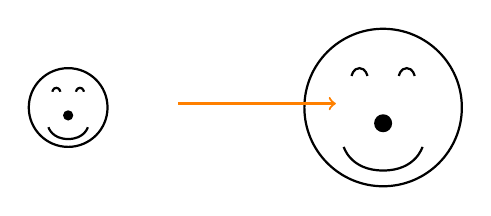
\begin{tikzpicture}[scale=0.5]
\draw[thick] (0cm,0cm) circle(1cm);
\draw[thick] plot [smooth,tension=1.5] coordinates{(-0.5,-0.5) (0,-0.8) (0.5,-0.5)};
\draw [thick, fill=black] (0,-0.2) circle (0.1);
\draw[thick] plot [smooth,tension=1.5] coordinates{(-0.4,0.4) (-0.3,0.5) (-0.2,0.4)};
\draw[thick] plot [smooth,tension=1.5] coordinates{(0.4,0.4) (0.3,0.5) (0.2,0.4)};
\draw[thick] (8cm,0cm) circle(2cm);
\draw[thick] plot [smooth,tension=1.5] coordinates{(7,-1) (8,-1.6) (9,-1)};
\draw [thick, fill=black] (8,-0.4) circle (0.2);
\draw[thick] plot [smooth,tension=1.5] coordinates{(7.2,0.8) (7.4,1) (7.6,0.8)};
\draw[thick] plot [smooth,tension=1.5] coordinates{(8.8,0.8) (8.6,1) (8.4,0.8)};
\draw[thick,->,orange](2.8,0.1)--(6.8,0.1) node[near start, above]{};
%\draw[thick,->,orange](5.8,-0.6)--(1.8,-0.6) node[near start, below]{Rotation by 90 degree counterclockwise};
\end{tikzpicture}Scalling

\vspace{0.3cm}


\begin{tikzpicture}[scale=0.5]
\draw[thick] (0cm,0cm) circle(1cm);
\draw[thick] plot [smooth,tension=1.5] coordinates{(-0.5,-0.5) (0,-0.8) (0.5,-0.5)};
\draw [thick, fill=black] (0,-0.2) circle (0.1);
\draw[thick] plot [smooth,tension=1.5] coordinates{(-0.4,0.4) (-0.3,0.5) (-0.2,0.4)};
\draw[thick] plot [smooth,tension=1.5] coordinates{(0.4,0.4) (0.3,0.5) (0.2,0.4)};
\draw[thick] (7,0)--(9,0);
\draw[thick,->,orange](2.8,0.1)--(6.8,0.1) node[near start, above]{};
%\draw[thick,->,orange](5.8,-0.6)--(1.8,-0.6) node[near start, below]{Rotation by 90 degree counterclockwise};
\end{tikzpicture}Projecting



\a\aa
In the space of functions, linear transformations happen when we \x{change variables} or make \x{linear combinations of functions}. For example, let $P_\infty$ be the space of all polynomials. The map defined by 
$$T: P_\infty  ⟶   P_\infty$$
$${f(x)  ↦ f(x^2)}$$ 

is \x{linear}, (\exe: Check it). 
\vfill
Remember to check that the expression $f(x^2)$ you defined is \x{actually} an element in the codomain. For example, if $P_2$ is the sapce of all polynomials of degree at most 2. The following argument
$$
T: P_2 ⟶   P_2$$
$$
f(x)↦  f(x^2)
$$
\x{is not even a map} ($x^2\mapsto x^4\notin P_2$)
\a\aa
You can also define linear transformation on set of functions by \x{linearly combine its function values}, \x{derivative}, or \x{integration} for example
$$
T:f(x)\mapsto f(1+\sqrt{x})+f(1-\sqrt{x});\qquad T:f(x)\mapsto xf(x)+x^2f(x)\quad $$$$T:f(x)\mapsto f'(x);\qquad T:f(x)\mapsto \int_0^x f(t)\dd t.
$$
\vfill
%The map $f\mapsto f'$ can be thought like linear combination of $f(x)$ with $f(x+0.01)$ with coefficient $-100f(x)+100f(x+0.01)$, but here in case of $f'$ the number $0.01$ and $100$ can be thought as replaced by infinitesimal and infinite numbers.


%\a{Linear space of linear transformation}
%Let $S$ be a set, $V$ a linear space, consider the set of all \x{maps}
%$$
%\Hom_{\mathrm{set}}(S,V):=\left\{f|f: S ⟶  V\right\}
%$$
%\vfill
%This set is \x{a linear space }under the following addition and scalar multiplication
%\vfill
%For any $f,g\in \Hom_{\mathrm{set}}(S,V)$ and $\lambda,\mu\in F$, $s\in S$
%$$
%(\lambda f+\mu g)(s):=\lambda f(s)+\mu g(s).
%$$
%\vfill
%\exe : Verify $\Hom_{\mathrm{set}}(S,V)$ is a linear space.
%\a\aa
%\exe Let $V,W$ be linear spaces over $F$, use the following symbol to denote the set all linear transformations from $W$ to $V$
%$$
%\mathcal L(W,V):=\left\{f|f: W ⟶  V \text{ linear transformation }\right\}
%$$
%We define addition and scalar multiplication for any $f,g\in \mathcal L(W,V)$ and $\lambda,\mu\in F$, $\ww\in W$ by
%
%$$
%(\lambda f+\mu g)(s):=\lambda f(s)+\mu g(s).
%$$
%
%Verify that $\mathcal L(W,V)$ is a linear space.
%
%\vspace{3cm}
\a{Verify a map is a linear transformation}
To verify a map $ T: V ⟶  W$ is a linear transformation, we only need
\vfill
\[itemize]{
\item Write down expression of $\vv_1,\vv_2$ for arbitrary element $\vv\in V$. 
\item Check the element is well-defined and it defined to be an element in codomain.
\item Compute $T(\lambda\vv_1+\vv_2)$ for arbitrary element $\lambda\in F$
\item Compare with $\lambda T(\vv_1)+T(\vv_2)$.
	}
We only verify $T(\lambda\vv_1+\vv_2)$ is because the following
\[prop]{For any map $T$, if $T(\lambda\vv_1+\vv_2)=\lambda T(\vv_1)+T(\vv_2)$, this is a linear tranformation.}
\[proof]{$T(\lambda\vv_1+\mu\vv_2)=\lambda T(\vv_1)+ T(\mu\vv_2)=\lambda T(\vv_1)+ \mu T(\vv_2)$}
\a\aa
\exe Let $P_2$ be the space of polynomials of degree at most 2. Show that the following map
$$
T: P_2 ⟶    P_2
$$
$$f(x) ↦ f(1+\sqrt x)+f(1-\sqrt x)
$$
is a linear transformation.

\sol Let $f,g$ be arbitrary polynomials in $P_2$, so there exists unique $a,b,c,d,e,f\in F$ so $f,g$ can be written as%\footnote{The use of \pa $a,b,c,d,e,f$  is an example of \enu}
\[equation]{\label{para}
f(x)=ax^2+bx+c\qquad g(x)=dx^2+ex+f.
}
We first show that $T[f]\in P_2$. Indeed,
$$
T[f](x)=f(1+\sqrt x)+f(1-\sqrt x)
$$
\a\aa

Plug \eqref{para} in, we have

$$
T[f](x)=a(1+\sqrt x)^2+b(1+\sqrt x)+c + a(1-\sqrt x)^2+b(1-\sqrt x)+c
$$

By computation, this expression equals to $$a(2+x^2)+2b+2c\in P_2.$$

\vfill
\vfill
To check linearity, note that for any scalar $\lambda\in f$
$$
T[\lambda f+g]=\lambda f(1+\sqrt x)+\lambda f(1-\sqrt x)+g(1+\sqrt x)+g(1-\sqrt x)=\lambda T[f]+T[g]
$$
So $T$ is a linear transformation.




\a{Non-linear transformations}
Non-linear transformations happens when we combine values of functions in a non-linear way, like $f(x)\mapsto f(x)^2$ or $f(x)\mapsto \sqrt{f(x)}$. To disprove linearity, we only need to choose some coefficient so that the definition of linear transformation fails to hold.
\vfill
Sometimes, we write $T[f]$ to denote the output function when apply linear transformation of $T$.
\a\aa
\exe Let $V$ be the space of all polynomials over $\RR$. Show that $T[f](x)=f(x)^2$ is not a linear transformation.
\vfill
\sol: Let $$\[cases]{f_1(x)=1\\f_2(x)=x}$$, then $$T[f_1+f_2](x)=(1+x)^2=1+x^2+2x$$
But
$$T[f_1](x)+T[f_2](x)=1+x^2.$$
So 
$$
T[f_1+f_2]\neq T[f_1]+T[f_2]
$$
This is not a linear transformation.

\aaa


\aaa{Matrix of linear transformations}
To represent a linear transformation, we will use matrices.
\a\aa
Shinchan is making drinks with the following recipe
\vfill
\[columns]{\co5
\t{}\cola\tea,\leaf11,\bean21.
\co5
\cola uses \fbox{\leaf\bean\bean}~\\
\vspace{2cm}
\tea uses \fbox{\leaf\bean}~\\
}
\a\aa
This time he would like to use pictures to organize the data. He plots each drink to the corresponding point in $\mathbb{R}^2$ to the linear combination space of materials.

\[columns]{\co7
\[z]{
\org
%\xaxis{-1}5
%\yaxis{-1}5
\grid{-3}{-3}33
%\wangge
\draw (1,0) node {\leaf} (0,1) node {\bean};
\draw (1,2) node {\cola} (1,1) node {\tea};
%\nnw A12
%\nnw B11
	}
\co3
\t{}\cola\tea,\leaf11,\bean21.
}
\a\aa
This process can be understood as a linear transformation \x{from the space of drink combinations} to \x{the space of material combinations}.



\t{}\cola\tea,\bean21,\leaf11.



\[columns]{
\co4

\[zz]{
\org
%	\pgftransformcm{1}{2}{1}{1}{\pgfpoint{0}{0}}
\grid[red!60!white!40]{-1}{-1}11
\draw[color=orange] (1,1) circle[radius=0.3] node {\sbento};
\draw[color=red] (0,1) circle[radius=0.3] node {\scola};
\draw[color=red] (1,0) circle[radius=0.3] node {\stea};
	}

\co1
$$\longrightarrow$$
\co5

\[zzz]{
\org
\grid{-3}{-3}33
\draw[color=blue] (1,0) circle[radius=0.3] node {\sleaf} (0,1) circle[radius=0.3] node {\sbean};
\draw[color=red] (1,2) circle[radius=0.3] node {\scola} (1,1) circle[radius=0.3] node {\stea};
\draw[color=orange] (2,3) circle[radius=0.3] node {\sbento};
	\pgftransformcm{1}{2}{1}{1}{\pgfpoint{0}{0}}
\grid[red!60!white!40]{-1}{-1}11
%\draw (1,1) node {\sbento};
	}


}


\a\aa
We call this map $T$. We use \cola, \tea as symbols for the drinks in the domain and 
$$T\left(\cola\right)\qquad T\left(\tea\right)$$ as symbols for its position in the codomain. Since materials are all in the codomain, it makes more sense to write our table as


\t{}{$T\left(\cola\right)$}{$T\left(\tea\right)$},\bean21,\leaf11.

\a\aa
This table can be written as an expression

$$
\m{T\cola}{T\tea}. = \m\bean\leaf. \m21,11.
$$

Factoring $T$ out we can write
$$
T\m{\cola}{\tea}. = \m\bean\leaf. \m21,11.
$$

Note that (\cola,\tea) is a basis of the domain, and (\bean,\leaf) is a basis of the codomain. We call the matrix
$$
\m21,11.
$$
The matrix representation of $T$ in the basis (\cola,\tea) and (\bean,\leaf). It determines the linear transformation completely.



\aaa






\aaa{Matrix Representation of a Linear Transformation}
The idea of matrix representation is to represent linear transformation as matrix. 

Look at the following example. Reflection vertically.
\vfill

\[columns]{
\co5
\[zzz]{
%\org
\grid{-3}{-3}33
%\draw[thick,->] (0,0) -- (1,0) node[right]{e_1};
%\draw[thick,->] (0,0) -- (0,1) node[right]{e_2};
\draw[thick] (0cm,0cm) circle(1cm);
\draw[thick] plot [smooth,tension=1.5] coordinates{(-0.5,-0.5) (0,-0.8) (0.5,-0.5)};
\draw [thick, fill=black] (0,-0.2) circle (0.1);
\draw[thick] plot [smooth,tension=1.5] coordinates{(-0.4,0.4) (-0.3,0.5) (-0.2,0.4)};
\draw[thick] plot [smooth,tension=1.5] coordinates{(0.4,0.4) (0.3,0.5) (0.2,0.4)};
}
\co5
\[zzz]{
%\org
\grid{-3}{-3}33
%\draw[thick,->] (0,0) -- (1,0) node[right]{e_1};
%\draw[thick,->] (0,0) -- (0,1) node[right]{e_2};
\draw[thick] (0cm,0cm) circle(1cm);
\draw[thick] plot [smooth,tension=1.5] coordinates{(-0.5,0.5) (0,0.8) (0.5,0.5)};
\draw [thick, fill=black] (0,0.2) circle (0.1);
\draw[thick] plot [smooth,tension=1.5] coordinates{(-0.4,-0.4) (-0.3,-0.5) (-0.2,-0.4)};
\draw[thick] plot [smooth,tension=1.5] coordinates{(0.4,-0.4) (0.3,-0.5) (0.2,-0.4)};
}
f
}
\a\aa
The idea is to fina a matrix to realize the action on all vectors by matrix multiplication. Clear, we find out that the formula for reflection vertically is given by
\[columns]{
\co5
\[zzz]{
\org
\grid{-3}{-3}33
\dian12
%\draw[thick]
}
\co5
\[zzz]{
\org
\grid{-3}{-3}33
\dian1{-2}
%\draw[thick]
}
}
The formula is mapping $\m x,y.$ to $\m x,{-y}.$.
\a\aa
However, this map can be written as a matrix multiplication.
$$
\underbrace{\m x,{-y}.}_{“new position“} = \m10,0{-1}.\underbrace{\m x,y.}_{“old position“}
$$
We call the matrix 
$$
\m10,0{-1}.
$$
The matrix representation of the linear transformation.
\a\aa
However, the notion of coordinate only make sense if we draw a grid, if we draw a different grid, the coordinate would change 
\[columns]{
\co4
\[zzz]{
\org
\grid{-3}{-3}33
\dian12
%\draw[thick]
}
\co4
\[zzz]{
\grid{-3}{-3}33
\dian1{-2}
\[scope]{[cm={sqrt(2)/2,-sqrt(2)/2,sqrt(2)/2,sqrt(2)/2,(0,0)}]
\org
\grid{-3}{-3}33
%\draw[thick]
}
}
}
\a\aa
For the following example, the coordinate of the right picture changes because we choose a different basis.
\[columns]{
\co4
\[zzz]{
\org
\grid{-3}{-3}33
\dian12
%\draw[thick]
}
\co4
\[zzz]{
\dian1{-2}
\[scope]{[cm={sqrt(2)/2,-sqrt(2)/2,sqrt(2)/2,sqrt(2)/2,(0,0)}]
\org
\grid{-3}{-3}33
%\draw[thick]
}
}
}

\a\aa
In linear algebra, a basis is the information of how to draw such a grid, 
\[columns]{
\co4
\[zzz]{
\org
\grid{-3}{-3}33
\draw[thick, ->] (0,0)--(1,0) node[right]{e_1};
\draw[thick, ->] (0,0)--(0,1) node[right]{e_2};
}

basis of domain
\co4
\[zzz]{
\dian1{-2}
\[scope]{[cm={sqrt(2)/2,-sqrt(2)/2,sqrt(2)/2,sqrt(2)/2,(0,0)}]
\org
\grid{-3}{-3}33
\draw[thick, ->] (0,0)--(1,0) node[right]{e_1};
\draw[thick, ->] (0,0)--(0,1) node[right]{e_2};
%\draw[thick]
}
}

basis of codomain
}

\a\aa
In general, the coordinate of a point can only be identified \x{after choosing a basis.} For example, 

\[zzz]{
\grid{-3}{-3}33
\draw[thick, ->] (0,0)--(1,0) node[right]{e_1};
\draw[thick, ->] (0,0)--(0,1) node[right]{e_2};
\dian12
}

The point is in fact given by $\vec v=\vec e_1+2\vec e_2 = \m{\vec e_1}{\vec e_2}.\m1,2.$

$$
\vec v = \underbrace{\m{\vec e_1}{\vec e_2}.}_{“Basis“}\underbrace{\m1,2.}_{“Coordinates“}
$$

\a\aa
In fact, the coordinate would change when choosing a different basis, 

\[columns]{
\co5
\[zzz]{
\grid{-3}{-3}33
\draw[thick, ->] (0,0)--(1,0) node[right]{e_1};
\draw[thick, ->] (0,0)--(0,-1) node[right]{e_2};
\dian12
}
\co5
\[zzz]{
\grid{-3}{-3}33
\draw[thick, ->] (0,0)--(1,0) node[right]{e_1};
\draw[thick, ->] (0,0)--(0,1) node[right]{e_2};
\dian12
}
}

$$
\vec v = \underbrace{\m{\vec e_1}{\vec e_2}.}_{“Basis“}\underbrace{\m1,2.}_{“Coordinates“}
= \underbrace{\m{\vec e_1}{-\vec e_2}.}_{“Basis“}\underbrace{\m1,{-2}.}_{“Coordinates“}
$$

\x{Coordinates depends on the choice of basis!}

\a\aa
For a linear transformation $T: V ⟶  W$, to represent vectors in $V$ and $W$, we need a basis $\obasis\ee n$ for $V$, and also a basis $\obasis\uu m$ for $W$. 

\a\aa
basis $\obasis\ee n$ for $V$; basis $\obasis\uu m$ for $W$.
\vfill
So we may write a vector $\vec v ∈ V$ and $T\vec v ∈ W$as
$$
\underbrace{\vec v = \obasis\ee n\coro xn}_{“Vector in “V} ↦ 
␣ 
\underbrace{T\vec v = \obasis\uu m \coro ym}_{“Vector in “W}
$$

A matrix representation of $T$ under the basis $\obasis\ee n$ and $\obasis\uu m$ means we want to find the matrix $M$ so that the fomula holds for all $\vec v$ 
$$
\coro ym = M \coro xn.
$$
\a\aa
Do such a formula exists? Yes, in fact

$$
T\obasis \ee n = \obasis{T\ee}n
$$
is a vector list in $W$, so we may find the list $M$ with each column collects the coordinate of $T\ee_i$ under the basis $\obasis\uu m$, so that one can write
$$
T\obasis\ee n = \obasis\uu m M.
$$
\a\aa
This $M$ is what we want, because
$$
T\underbrace{\obasis\ee n\coro xn}_{\vec v} = \obasis\uu mM\coro xn
$$
On the other hand, we want
$$
T\vec v = \obasis\uu m\coro ym,
$$
\a\aa
This implies that
$$
\obasis\uu mM\coro xn = \obasis\uu m\coro ym
$$
Since linearly independent vectors have left-inverse, we cancel it from left and have
$$
M\coro xn = \coro ym.
$$


\a\aa
\[defi]{For a linear transformation $T: V ⟶  W$, let 
\[itemize]{
\item $\ce=\obasis\ee n$ be a basis of domain $V$
\item $\cw=\obasis\uu m$ be a basis of codomain $W$. 
}The \x{matrix representation} of $T$ with respect to $\ce$ and $\cw$, is the matrix $P$ such that
$$
T\obasis\ee n=\obasis\uu m P
$$
%We denote by $P=\nota T\ce\cw$
}
In other words, the matrix representation is the recipe table to make $T\obasis\ee n$ by materials $\obasis\uu m$.
\vfill
Note: Different basis will result different matrix representation for the same linear transforamtion $T : V ⟶  W$!
\a\aa
%The matrix representation $P$ of $T: V ⟶  W$ with basis $\ce$ and $\cw$, is the coordinate matrix of
%$$
%T\ce=\obasis{T\ee}n
%$$
%in the following basis of codomain $W$
%$$
%\cw = \obasis\ww m.
%$$
%The matrix $P$ fits into the following linear combination equation
%$$
%\overbrace{\obasis{T\ee}n}^{T\ce} = \overbrace{\obasis\ww m}^{\cw}P 
%$$
%Each column of $P$ is the coordinate of $T\ee_i$ in the \bas $\cw$.
%$$
%P=\m{\nota{T\ee_1}{}\cw}{\nota{T\ee_2}{}\cw}\cdots{\nota{T\ee_n}{}\cw}.
%$$
%\a\aa
\exe Let $V=\lPP xabc$, $W=\lPP tabc$

Consider a linear map 
$$T: V ⟶  W   $$$${f(x) ↦ f(t+1)}$$

Find matrix representation of $T$ with bases 
$$\cw=\m1t{t^2}.\text{ in }W\qquad \ce=\m1{2x+1}{x^2+1}.\text{ in }V$$
\a\aa
\sol: Apply the \lt $T$ on each of the function on \bas and write the coordinate in \bas of the target.
We find 
\[equation*]{\[split]{
	T(1)=1 &={\underbrace{\m1t{t^2}.}_\cw\underbrace{\m1,0,0.}_{}}\\
T(2x+1)=2(t+1)+1 &={\underbrace{\m1t{t^2}.}_\cw\underbrace{\m3,2,0.}_{}}\\
T(x^2+1)=(t+1)^2+1&={\underbrace{\m1t{t^2}.}_\cw\underbrace{\m2,2,1.}_{}}
}
}
\a\aa
We write this into a matrix form
$$
T\underbrace{\m1{2x+1}{x^2+1}.}_\ce=\underbrace{\m1t{t^2}.}_\cw\m132,022,001.
$$

We know the matrix representation of $T$ is $ \m132,022,001.$
\a\aa
\exe For the map 
$$T: V ⟶  W   $$$${f(x) ↦ f(t+1)}$$ the matrix representation has been found
$$T\underbrace{\m1{2x+1}{x^2+1}.}_{“ basis in “V} = \underbrace{\m1t{t^2}.}_{“ basis in “W}\m132,022,001.$$
Suppose $f(x) = 3+5(2x+1)+2(x^2+1)$, use your matrix, find $Tf$
\a\aa
\sol We find the coordinate of $f$ is just $\m3,5,2.$ Therefore, the coordinate of $Tf$ in codomain is just obtained by multiplying the matrix to the coordinate of $f$ in domain, we get
$$
\m132,022,001.\m3,5,2.
=\m{22},{14},2.
$$
Therefore $Tf = \m1t{t^2}.\m{22},{14},2.  = 22+14t+2t^2$.

\a\aa
\sol You may also proceed by the standard notation
$$
Tf = T\m1{2x+1}{x^2+1}.\m3,5,2. = \m1t{t^2}.\m132,022,001.\m3,5,2.$$
$$ = \m1t{t^2}.\m{22},{14},2.  = 22+14t+2t^2.
$$
\aaa









\aaa{Polynomials on Linear Operators}
From now we only consider the linear operators which is transformations with the same domain and codomain. $T: V ⟶  V$
\vfill
When represnting the matrix of this linear transformation, we keep the basis in domain and codomain the same. So only one choice of basis is required.
\a\aa
\exe Represent the matrix of taking derivative $T: P_3   ⟶  P_3$with respect to the basis $\m 1t{t^2}{t^3}.$

$$
T\m 1t{t^2}{t^3}. = \m {T(1)}{T(t)}{T(t^2)}{T(t^3)}.
$$

$$
=\m01{2t}{3t^2}.
$$

$$
=\m 1t{t^2}{t^3}.\underbrace{\m0100,0020,0003,0000.}_{“matrix represntation of “T “ under basis “}
$$
\vfill
\a\aa
Since domain and codomain are the same, we must choose the same basis both in domain and codomain.
$$
T\underbrace{\m 1t{t^2}{t^3}.}_{“choice of basis of domain“}=\underbrace{\m 1t{t^2}{t^3}.}_{“must be the same “}\underbrace{\m0100,0020,0003,0000.}_{“matrix represntation of “T “ under basis “}
$$



\a\aa
Linear Operator $T: V ⟶  V$ can be raise into powers. By
$$
T^n:=\underbrace{T\circ T\circ\cdots\circ T}_{n\text{ many }T}
$$
This is the \emph{$n$-th power} of the operator $T$. Using this notion of (integer) powers, we can define many new operators on $V$ given by \emph{polynomials}. For example we can define things like
$$
T^2+2T+\id_V
$$
You will find it is exactly equal to the operator
$$
(T+\id_V)^2.
$$
For our convenience, we abbreviate $\id_V$ as $I$.
\a\aa
The algebra of linear operators can be concretly evaluated on its matrix representations. Because if $ℰ $ is a basis and $A$ is the matrix of $T$ under $ℰ $, in other words, $Tℰ =ℰ A$, then
$$
T^n ℰ  = T^{n-1} ℰ A = T^{n-2} ℰ A² = ... = ℰ A^n
$$

\vfill

In other words, under the same basis, if matrix representation of $T$ is given by $A$, then the matrix represenrtation of $T^n$ is given by $A^n$.
\a\aa
In general we can apply a polynomial of degree $m \in \mathbb{N}$
$$
p(x)=a_mx^m+a_{m-1} x^{m-1}+\cdots+a_0
$$
to the operator $T$ by evaluating $P$ at $x=T$, obtaining
$$
p(T):=a_mT^m+a_{m-1} T^{m-1}+\cdots+a_0 \cdot I
$$
\a\aa
\exe Suppose $T$ is a linear operator on $V$ such that 
$$
(T-I)^2=0.
$$
Show that $T$ is invertible.
\vfill
\textbf{Proof.}
We have $T^2-2T+I=0$, therefore $-T^2+2T=I$, so $T(2-T)=I$. This implies $T$ is invertible and 
$$
T^{-1}=2-T.
$$
\aaa


